\documentclass[20pt, a0paper, portrait, margin=15mm, innermargin=15mm,
     blockverticalspace=15mm, colspace=15mm, subcolspace=8mm]{tikzposter} %Default values for poster format options.

\tikzposterlatexaffectionproofoff %hides small comment on how the poster was made at bottom of poster

% \renewcommand{\tiny}{\fontsize{1}{26.5}\selectfont}
% \renewcommand{\scriptsize}{\fontsize{26.5}{32}\selectfont}
% \renewcommand{\footnotesize}{\fontsize{31}{38}\selectfont}
% \renewcommand{\small}{\fontsize{25}{30}\selectfont}
% \renewcommand{\normalsize}{\fontsize{25}{30}\selectfont}
% \renewcommand{\large}{\fontsize{25}{30}\selectfont}
% \renewcommand{\Large}{\fontsize{66}{73}\selectfont}
% \renewcommand{\LARGE}{\fontsize{80}{95}\selectfont}
% \renewcommand{\huge}{\fontsize{96}{115}\selectfont}
% \renewcommand{\Huge}{\fontsize{80}{96}\selectfont}

%% +++++ Packages ++++++
% Writing and font related
\usepackage[utf8]{inputenc} % encoding
\usepackage{exscale} 
%% +++++  Custom Packages ++++++
\usepackage{bm}
\usepackage{graphicx}
\usepackage{tikz} 
\usepackage{color}
\usepackage{xcolor}
\usepackage{listings}
\usepackage[absolute]{textpos}
\usepackage{inputenc}
\usepackage{layout}
\usepackage{nameref}
\usepackage{float}
\usepackage{tabularx}
\usepackage[export]{adjustbox}
\usepackage{subcaption}
\usepackage{wrapfig}
\usepackage{bm}
\usepackage{bbold}
\usepackage{changepage}
%\usepackage[labelformat=empty]{caption}
\usepackage{caption}
%% +++++ Custom Packages End ++++++
\usepackage{sfmath}  % Sans-serif math font
\renewcommand{\familydefault}{\sfdefault}
\usepackage{scalerel}
\usepackage{relsize}
% Programming
\usepackage{xspace}
\usepackage{xargs}
\usepackage{ifthen}
\usepackage{etoolbox}
% Math
\usepackage{amsmath} % For typesetting math
\usepackage{amssymb} % Adds new symbols to be used in math mode
%\usepackage{amsfonts}
%\usepackage{mathrsfs}
%\usepackage{dsfont}
%\usepackage{amsthm}
%\usepackage{thmtools}
\usepackage[fixamsmath,disallowspaces]{mathtools}
% Misc
\usepackage{array}
\usepackage{enumitem}
\usepackage{adjustbox}
\usepackage{url}
\usepackage{lipsum}
\pdfminorversion=7

%% +++++ Custom Commands ++++++
% Add your custom commands here
\newcommand{\va}[1]{\bm{#1}}
\newcommand{\ta}[1]{\bm{#1}}
%\newcommand{\tave}[1]{\langle #1 \rangle_t}
\newcommand{\tave}[1]{\overline{#1}}
\newcommand{\txv}[0]{ \,}
\newcommand{\p}[0]{\partial}
\newcommand{\mtxt}[1]{\textrm{#1}}
\newcolumntype{C}[1]{>{\hsize=#1\hsize\centering\arraybackslash}X}%
\newcommand{\plot}[3]{
\begin{figure}[H]
    \centering
    \scriptsize
    %\tiny
    \scalebox{1.3}{\input{#1}}
    \caption{\footnotesize{#2}}
    \label{#3}
\end{figure}
}

% Math Macros
%%% --> Braces and Annotations <--
% braces for operators (removes the spacing before and after the delimiters)
\newcommand{\opleft}[1]{\mathopen{}\left#1}
\newcommand{\opright}[1]{\right#1\mathclose{}}
% flexible brace command, #1=left delimiter, #2=right delimiter, #3=size (normal, auto, opauto, \[sizecmd]), #4=content
\newcommandx{\braces}[4]{%
\ifstrequal{#3}{normal}{#1#4#2}{%
\ifstrequal{#3}{auto}{\left#1#4\right#2}{%
\ifstrequal{#3}{opauto}{\opleft#1#4\opright#2}{%
#3#1#4#3#2}}}%
}
% annotation on the top of relation symbols
\newcommandx{\opannot}[3][3=\downarrow]{\stackrel{\mathclap{\substack{#1 \\ #3 \vspace{2pt}}}}{#2}}
% annotation in front of a line
\newcommandx{\lineannot}[3][3=\rightarrow]{\mathllap{\boxed{\text{\textsmaller{#1}}} #3} #2}
% annotation in front of a line (multiline)
\newcommandx{\multilineannot}[4][4=\rightarrow]{\mathllap{\boxed{\parbox{#1}{\RaggedRight\textsmaller{#2}}} #4} #3}
% annotation between two lines
\newcommand{\interannot}[1]{\boxed{\text{\textsmaller{#1}}}} 
% annotation between two lines (multiline)
\newcommand{\multiinterannot}[2][.5\textwidth]{\boxed{\parbox{#1}{\RaggedRight\textsmaller{#2}}}}

%%% --> Number Sets and Symbols <--
\newcommand{\N}{\mathbb{N}} % natural numbers
\newcommand{\Nzero}{\mathbb{N}_0} % natural numbers with zero
\newcommand{\Z}{\mathbb{Z}} % integer numbers
\newcommand{\Q}{\mathbb{Q}} % rational numbers
\newcommand{\R}{\mathbb{R}} % real numbers
\newcommand{\Rpos}{\mathbb{R}_{>0}} % positive real numbers
\newcommand{\C}{\mathbb{C}} % complex numbers
\newcommand{\K}{\mathbb{K}} % field (real or complex numbers)
\newcommand{\eps}{\varepsilon} % shortcut for epsilon
\renewcommand{\Re}{\operatorname{Re}}
\renewcommand{\Im}{\operatorname{Im}}

%%% --> Logic <--
\renewcommand{\iff}{\Leftrightarrow} % if and only if
\renewcommand{\implies}{\Rightarrow} % implies
\newcommand{\suchthat}[1][normal]{\ifstrequal{#1}{normal}{\mid}{#1|}} % seperator in sets (#1op = size)

%%% --> Sets and Topology <--
\newcommand{\setcompl}[1]{#1^c} % complement of a set
\newcommand{\cardinality}{\#} % cardinality of a set
\newcommand{\union}{\cup} % union
\newcommand{\disjunion}{\mathrel{\dot{\union}}} % disjoint union
\newcommand{\bigunion}{\bigcup} % big union
\newcommand{\bigdisjunion}{\mathop{\dot{\bigcup}}} % big disjoint union
\newcommand{\intersec}{\cap} % intersection
\newcommand{\bigintersec}{\bigcap} % big intersection
\newcommand{\boundary}[1]{\partial#1} % boundary of a set
\newcommand{\clos}[1]{\overline{#1}} % topological closure of a set
\newcommand{\interior}[1]{\mathring{#1}} % interior of a set
\newcommand{\dist}[2]{\operatorname{dist}(#1, #2)} % distance between two sets

%%% --> Analysis <--
\newcommandx{\intvcl}[3][1=normal]{\braces{[}{]}{#1}{#2, #3}} % closed interval (#1op=size, #2=left bound, #3=right bound)
\newcommandx{\intvop}[3][1=normal]{\braces{(}{)}{#1}{#2, #3}} % open interval
\newcommandx{\intvclop}[3][1=normal]{\braces{[}{)}{#1}{#2, #3}} % half-open interval (right)
\newcommandx{\intvopcl}[3][1=normal]{\braces{(}{]}{#1}{#2, #3}} % half-open interval (left)
\newcommand{\dotarg}{\ensuremath{\raisebox{.15ex}{$\scriptstyle [\cdot]$}}} % a dot, where a variable could be put into
\DeclareMathOperator*{\argmin}{argmin} % argmin
\DeclareMathOperator*{\argmax}{argmax} % argmax
\DeclareMathOperator{\sign}{sign}
\newcommandx{\abs}[2][1=normal]{\braces{\lvert}{\rvert}{#1}{#2}} % absolute value
\newcommand{\conj}[1]{\overline{#1}} % complex conjugation
\newcommandx{\ceil}[2][1=normal]{\braces{\lceil}{\rceil}{#1}{#2}} % ceil
\newcommandx{\floor}[2][1=normal]{\braces{\lfloor}{\rfloor}{#1}{#2}} % floor
\newcommandx{\round}[2][1=normal]{\braces{[}{]}{#1}{#2}} % round
\newcommandx{\der}[1]{D^{#1}} % differential operator (#1 = multiindex)
\newcommandx{\partder}[4][1={},4={}]{\frac{\partial^{#4} #2}{\partial #3^{#4}}\ifargdef{#1}{\Big|_{#1}}} % partial derivative (#1=point of evaluation, #2=function, #3=variable, #4=order)
\newcommandx{\integ}[4][1={},2={}]{\int_{#1}^{#2} #3 \, #4} % integral (#1op=lower bound, #2op=upper bound, #3=integrand, #4=differential form)
\newcommandx{\asympffaster}[2][1=normal]{o\braces{(}{)}{#1}{#2}} % asymptotically faster (proper) (#1op=size)
\newcommandx{\asympfaster}[2][1=normal]{O\braces{(}{)}{#1}{#2}} % asymptotically faster
\newcommandx{\asympeq}[2][1=normal]{\Theta\braces{(}{)}{#1}{#2}} % asymptotically equal
\newcommandx{\asympsslower}[2][1=normal]{\omega\braces{(}{)}{#1}{#2}} % asymptotically slower (proper)
\newcommandx{\asympslower}[2][1=normal]{\Omega\braces{(}{)}{#1}{#2}} % asymptotically slower

%%% --> Linear Algebra and Functional Analysis <--
\DeclareMathOperator{\Id}{Id} % identity operator
\newcommand{\GL}[2]{\operatorname{GL}(#1, #2)} % general linear group (#1=dimension, #2=field)
\newcommand{\matr}[1]{\begin{bmatrix} #1 \end{bmatrix}} % matrix
\newcommand{\smallmatr}[1]{\left[\begin{smallmatrix} #1 \end{smallmatrix}\right]} % small matrix
\newcommandx{\norm}[2][1=normal]{\braces{\|}{\|}{#1}{#2}} % norm
\renewcommandx{\sp}[3][1=normal]{\braces{\langle}{\rangle}{#1}{#2, #3}} % inner product (#1op=size, #2=left, #3=right)
\newcommand{\adj}[1]{{#1}^\ast} % adjoint operator
\newcommandx{\End}[2][2={}]{\mathcal{L}\opleft( #1 \ifargdef{#2}{, #2} \opright)} % endomorphism (#1=from, #2op=to)
\newcommand{\orthsum}{\oplus} % orthogonal sum
\newcommand{\orthcompl}[1]{{#1}^\perp} % orthogonal complement
\newcommand{\tensprod}{\otimes} % tensor product
\DeclareMathOperator{\ran}{ran} % image/range
% \DeclareMathOperator{\ker}{ker} % Kern
\DeclareMathOperator{\spann}{\operatorname{span}} % span
\newcommand{\T}{\top} % transposition (of a matrix)
\newcommand{\embeds}{\hookrightarrow} % embedding
\renewcommand{\vec}[1]{\boldsymbol{#1}} % vectors in boldface

%%% --> Function Spaces <--
% \newcommand{\almostev}{\text{f.ü.}} % fast überall
\newcommand{\almostev}{\text{a.e.}} % almost everywhere
\newcommandx{\measure}[2][1=normal]{\operatorname{vol}\braces{(}{)}{#1}{#2}} % Lebesgue-measure/volume of a set
\newcommand{\indset}[1]{\chi_{#1}} % indicator function for sets
\newcommand{\indcoeff}[1]{\mathds{1}_{#1}} % indicator function for sequences
\DeclareMathOperator{\supp}{supp} % support
\newcommandx{\Leb}[3][1={},3=normal]{L^{#2}\ifargdef{#1}{\braces{(}{)}{#3}{#1}}{}} % Lebesgue spaces (#1op=set, #2=exponent)
\newcommandx{\Lebnorm}[4][1=normal,3={2},4={}]{\norm[#1]{#2}_{#3}} % Lebesgue norm (#1op=size, #2=content, #3op=exponent, #4op=set)
\renewcommandx{\l}[3][1={},3=normal]{\ell^{#2}\ifargdef{#1}{\braces{(}{)}{#3}{#1}}} % lp sequence spaces (#1op=set, #2=exponent)
\newcommandx{\lnorm}[4][1=normal,3={2},4={}]{\norm[#1]{#2}_{#3}} % lp norm (#1op=size, #2=content, #3op=exponent, #4op=set)
\newcommandx{\Smooth}[4][1={},3={},4=normal]{C_{#3}^{#2}\ifargdef{#1}{\braces{(}{)}{#4}{#1}}} % space of differentiable functions (#1op=set, #2=order, #3op=modifier)
\newcommandx{\Schwartz}[2][1={},2=normal]{\mathscr{S}\ifargdef{#1}{\braces{(}{)}{#2}{#1}}} % space of Schwartz functions
\newcommandx{\Schwartzpoly}[2][1=normal]{\braces{\langle}{\rangle}{#1}{\abs[#1]{#2}} } % Schwartz polynomial
\newcommand{\Schwartznorm}[3]{C_{#1,#2}(#3)} % Schwartz space norm
\newcommandx{\Tempdistr}[2][1={},2=normal]{\mathscr{S}'\ifargdef{#1}{\braces{(}{)}{#2}{#1}}} % tempered distributions
\newcommandx{\distrinp}[3][1=normal]{\braces{\langle}{\rangle}{#1}{#2, #3}} % evaluation of a tempered distribution (#1op=size, #2=distribution, #3=Schwartz function)
\newcommand{\Linedistr}[1][]{\mathfrak{L}\ifargdef{#1}{_{#1}}{}} % line distribution
\newcommand{\conv}{\star} % convolution operator
\newcommandx{\ft}[3][1=default,2=auto]{
\ifstrequal{#1}{default}{\widehat{#3}}{
\ifstrequal{#1}{long}{{\braces{(}{)}{#2}{#3}}^{\wedge}}{}}} % Fourier transform (hat-notation) (#1op=long expression mode, #2op=size, #3=content)
\newcommand{\ftop}{\mathcal{F}} % Fourier transform (operator notation)
\newcommandx{\ift}[3][1=default,2=auto]{
\ifstrequal{#1}{default}{\check{#3}}{
\ifstrequal{#1}{long}{{\braces{(}{)}{#2}{#3}}^{\vee}}{}}} % inverse Fourier transform (hat-notation) (#1op=long expression mode, #2op=size, #3=content)
\newcommand{\iftop}{\mathcal{F}^{-1}} % inverse Fourier transform (operator notation)

%%% --> Miscellaneous <--
\newcommand{\sinc}{\operatorname{sinc}} % sinc function

%% +++++ Title and Author ++++++
\newcommand{\mytitle}{Statistical properties of material line elements in incompressible MHD turbulence}
\newcommand{\myauthor}{Philipp Hess, Oliver Henze, Wolf-Christian Müller \\\vspace{1cm} Zentrum für Astronomie und
Astrophysik, Technische Universität Berlin, Germany}
		
%% +++++ Predefined Daedalus Theme ++++++
%% +++++ Definition of Colors ++++++
\definecolor{lightblue}{rgb}{0.145,0.6666,1} % Defines the color used for content box headers
\definecolor{darkred}{rgb}{.65,0,0}
\definecolor{darkgreen}{rgb}{0,0.65,0}
% \definecolor{frameborder}{rgb}{0.035,0.313,0.62}
% \definecolor{lightblue}{rgb}{.5,0,0}
\definecolor{daedalusblue}{RGB}{0,80,160}
\definecolor{lightblue}{RGB}{215,224,249}
\definecolor{lightgreen}{RGB}{224,249,215}
\definecolor{grey}{rgb}{.5,.5,.5}

%% +++++ Color Style ++++++
\definecolorstyle{Daedalus}{
	\definecolor{colorOne}{named}{lightblue}
	\definecolor{colorTwo}{named}{yellow}
	\definecolor{colorThree}{named}{daedalusblue}
}{
	% Background Colors
	\colorlet{backgroundcolor}{white}
	\colorlet{framecolor}{black}
	\colorlet{frameborder}{colorThree!80}
	% Title Colors
	\colorlet{titlefgcolor}{colorThree}
	\colorlet{titlebgcolor}{colorOne}
	% Block Colors
	\colorlet{blocktitlebgcolor}{colorThree!80}
	\colorlet{blocktitlefgcolor}{white}
	\colorlet{blockbodybgcolor}{white}
	\colorlet{blockbodyfgcolor}{black}
	% Innerblock Colors
	\colorlet{innerblocktitlebgcolor}{white}
	\colorlet{innerblocktitlefgcolor}{black}
	\colorlet{innerblockbodybgcolor}{colorOne}
	\colorlet{innerblockbodyfgcolor}{black}
	% Note colors
	\colorlet{notefgcolor}{black}
	\colorlet{notebgcolor}{colorTwo!50!white}
	\colorlet{noteframecolor}{colorTwo}
}

%% +++++ Title Style ++++++
\definetitlestyle{Daedalus}{width=.96\textwidth, roundedcorners=10, linewidth=8pt, innersep=1cm,
    titletotopverticalspace=15mm, titletoblockverticalspace=20mm,
    titlegraphictotitledistance=10pt, titletextscale=2
}{
    \begin{scope}[line width=\titlelinewidth, rounded corners=\titleroundedcorners]
        \draw[color=frameborder]%
        (\titleposleft,\titleposbottom) rectangle (\titleposright,\titlepostop);
    \end{scope}
}
% Title + Logos
\settitle{ \quad
\begin{minipage}{13cm}
    \textcolor{white}{dummy}
%
\includegraphics[width=6cm]{images/daedalus_en_verlauf_rgb_72dpi.png}
\end{minipage}
\begin{minipage}{.69\linewidth}
\color{titlefgcolor}
\centering
{\bfseries \Huge \mytitle \par} 

\vspace{1.5\baselineskip}
{\huge \myauthor}
\end{minipage}\qquad
\hfill
\begin{minipage}{13cm}
\centering

\includegraphics[height=3.5cm]{images/TU_Logo_lang_RGB_rot.png} \quad
\end{minipage}
}

%% +++++ Block Style ++++++
\defineblockstyle{Daedalus}{
    titlewidthscale=1, bodywidthscale=1, titlecenter,
    titleoffsetx=0pt, titleoffsety=0pt, bodyoffsetx=0pt, bodyoffsety=15mm,
    bodyverticalshift=15mm, roundedcorners=10, linewidth=4pt,
    titleinnersep=8mm, bodyinnersep=16mm
}{
    \draw[rounded corners=\blockroundedcorners, inner sep=\blockbodyinnersep, line width=\blocklinewidth, color=frameborder, fill=blockbodybgcolor]
        (blockbody.south west) rectangle (blockbody.north east); %
    \ifBlockHasTitle%
        \draw[rounded corners=10, inner sep=\blocktitleinnersep, line width=\blocklinewidth, color=frameborder, fill=blocktitlebgcolor]
			(blocktitle.south west) rectangle (blocktitle.north east); %
    \fi%
}

%% +++++ Inner Style ++++++
% \defineinnerblockstyle{Daedalus}{
%     titlewidthscale=1, bodywidthscale=1, titlecenter,
%     titleoffsetx=0pt, titleoffsety=0pt, bodyoffsetx=0pt, bodyoffsety=0pt,
%     bodyverticalshift=0pt, roundedcorners=5, linewidth=1.5mm,
%     titleinnersep=.5em, bodyinnersep=1em
% }{
%     \begin{scope}[line width=1pt, rounded corners=\innerblockroundedcorners]
%        \ifInnerblockHasTitle %
%            \draw[fill=innerblockbodybgcolor]
%                (innerblockbody.south west) rectangle (innerblocktitle.north east);
%            \draw[color=black]
%                (innerblocktitle.south west) -- (innerblocktitle.south east);%
%        \else
%              \draw[draw=none, fill=innerblockbodybgcolor]
%                  (innerblockbody.south west) rectangle (innerblockbody.north east);
%         \fi
%     \end{scope}
% }

%% +++++ Setup Layout ++++++
\definelayouttheme{Daedalus}{
    \usecolorstyle{Daedalus}
    \usebackgroundstyle{Default}
    \usetitlestyle{Daedalus}
    \useblockstyle{Daedalus}
    \useinnerblockstyle{Default}
    \usenotestyle{Default}
}

%% +++++ Custom Commands ++++++
% Vertical space used before and after certain environments
\newcommand{\skippar}{\vspace{.5\baselineskip}}

% Custom headers
\newcommand{\subheader}[1]{\skippar\centerline{\color{colorThree!80}\Large\textbf{#1}}\skippar}
\newcommand{\inlineheader}[1]{{\color{blue}\textbf{#1}}}
% Highlighted text commands
\newcommand{\highlight}[1]{{\color{red}\sffamily\textbf{#1}}}
\newcommand{\defined}[1]{{\color{darkgreen}\textbf{#1}}}
\newcommand{\important}[1]{{\color{red}\textbf{#1}}}
% Custom itemize environment
\newenvironment{itemsposter}{\skippar\begin{itemize}[label={\color{colorThree!80}$\blacktriangleright$},leftmargin=1.5em,topsep=6pt,itemsep=0em,parsep=0pt,labelsep=.5em]}{\end{itemize}\skippar}
% Custom boxed frames
\newcommand{\definebox}[1]{\skippar\coloredbox[innersep=1em,linewidth=1pt,framecolor=black,roundedcorners=0,bgcolor=colorOne,roundedcorners=5]{#1}\skippar}
\newcommand{\makeframe}[3]{\skippar\coloredbox[width=#1,innersep=.5em,linewidth=1pt,framecolor=black,roundedcorners=0,bgcolor=#2,roundedcorners=5]{#3}\skippar}

\usetheme{Daedalus}

\begin{document}

	\maketitle

%% +++++ Left column ++++++

	\begin{columns}%blocks will be placed into columns
	\column{.4}

       \block{Background}{
        The deformation of material lines in turbulence is of fundamental interest and
        practical importance. Due to its diffusive character material lines
        consisting of the same set of fluid particles tend to stretch while following the
        fluid motion. Vortex lines and magnetic field lines in an inviscid fluid
        of high conductivity are examples of vector fields that are proportional to
        material lines. It is  known analytically [\,1\,] and shown in hydrodynamic
        simulations [\,2\,][\,3\,] that the length of material line elements
        increases exponentially in time. In the present work the deformation of
        material lines is studied statistically by simulating infinitesimal
        material line elements 
        in stationary incompressible magnetohydrodynamic (MHD) turbulence using
        velocity gradient time series. The velocity gradient data is obtained by tracking
        Lagrangian particles in a stochastically forced direct numerical simulation (DNS).
        In order to further understand the influence of the magnetic field on the material
        line deformation a method for injecting cross helicity has been devised to control
        the alignment of the magnetic and velocity field.
      }


      \block{Material line elements simulation}{

	  	A material line is defined as a line that always consists of the same set of particles or fluid
		elements. In order to study the material line dynamics statistically the lines are simplified to 
		infinitessimal elements (Batchelor $[1]$) which allows for a one-point description. 

		%\begin{figure}[H]
		\vspace{2cm}
		\begin{center}
        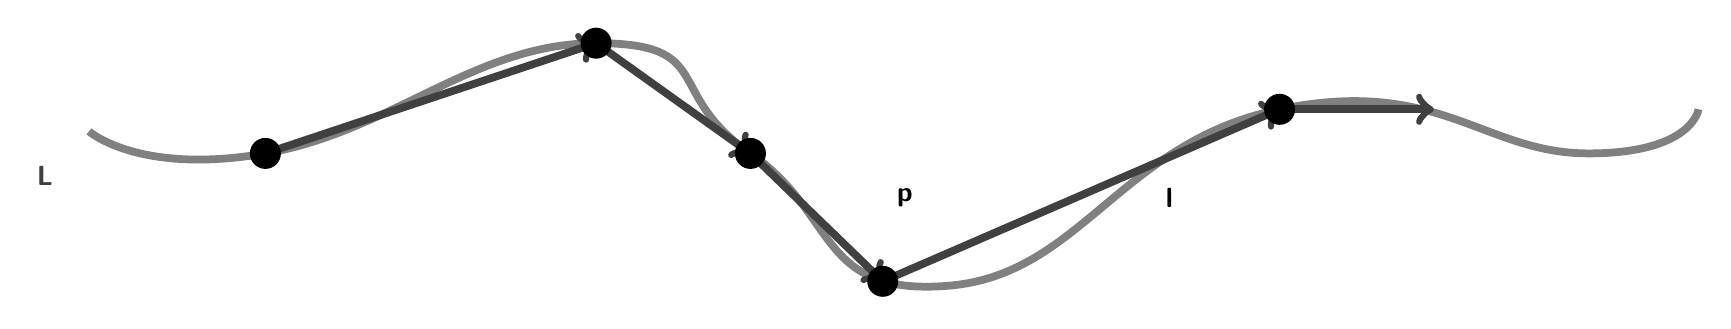
\begin{tikzpicture}[scale=2.8]

            \tikzset{ultra thick/.style={line width=2.8pt}}

            \draw [gray, ultra thick ] plot [smooth, tension=0.9] coordinates {
            (-3.8, 0.1) (-3., 0.0) (-1.5, 0.5) (-0.8, -0.0)
            (0.1, -0.6) (1.6, 0.2) (3.0,  0.0) (3.5,  0.2)};


            \draw[ultra thick, darkgray,->] (-3. , 0.0) -- (-1.5, 0.5);
            \draw[ultra thick, darkgray,->] (-1.5, 0.5) -- (-0.8,-0.0);
            \draw[ultra thick, darkgray,->] (-0.8,-0.0) -- (-0.2,-0.58);
            \draw[ultra thick, darkgray,->] (-0.2,-0.58) -- (1.6, 0.2);
            \draw[ultra thick, darkgray,->] (1.6, 0.2) -- (2.3, 0.2);
              
            \fill (-3.0, 0.0)  circle[radius=2pt];
            \fill (-1.5, 0.5)  circle[radius=2pt];
            \fill (-0.8,-0.0 )  circle[radius=2pt];
            \fill (-0.2,-0.58)  circle[radius=2pt];
            \fill (1.6,0.2)  circle[radius=2pt];

			\node [darkgray] at (-4.0 ,-0.1) {\textbf{L}};
            \node [black] at (1.1, -0.2) {$\va{l}$};
            \node [black] at (-0.1, -0.2) {$\va{p}$};
  
        \end{tikzpicture}
		\vspace{1cm}
		\captionof{figure}{A material line $L$ is approximated by line elements $l$ which are computed for
        for each lagrangian particle $p$.}
		\end{center}
		\vspace{2cm}
		%\caption{a line} 
		%\label{fig:line}
		%\end{figure}	
		The dynamical evolution of a line element $\va{l}$ is given by
       
       \begin{equation}
           \frac{d \va{l}}{d t} = \nabla \va{u} \, \va{l} =
           \ta{S} \txv \va{l} + \ta{\Omega} \txv \va{l},
       \end{equation}
	   where velocity gradient can be split into is the symmetric part $\ta{S}$ (strain-rate tensor) 
	   and an antisymmetric part $\ta{\Omega}$(rotation-rate tensor). The line stretching rate $\zeta$ is defined as

       \begin{equation}
           \label{zeta}
           \zeta \equiv \frac{d \ln(l)}{d t} = S_{ij} \hat{l}_i  \hat{l}_j.
           %\qquad \xi \equiv \frac{d \ln(A)}{d t} = -S_{ij} \hat{n}_i
           %\hat{n}_j, \; \va{A} = \va{l_1} \times \va{l_2}
       \end{equation}

       In the simulation lagrangian velocity gradient data $\va{V}$ is first gathered for each particle
	   and then used to evolve the corresponding line elements through the matrix $\va{M}$

        \begin{equation}
            \frac{d}{dt} \va{M} = \va{V} \txv \va{M}(t), \qquad \va{M}(0) = \mathbb{1},
        \end{equation}

        \begin{equation}
            \va{l}(t) = \va{M}(t) \txv \va{l}(0).
        \end{equation}

	}

       \block{Forcing Method}{

        The velocity gradient is obtained by tracking lagrangian particles through
        tricubic interpolation in a direct numerical simulation of the 
        incompressible MHD equations, 

        \begin{equation}
        \begin{aligned}
            \partial_t \va{\omega} &= \nabla \times [\va{v} \times \va{\omega}
            - \va{B} \times (\nabla \times \va{B})] + \nu \nabla^{2} \va{\omega}
            + \va{F}_{\va{\omega}}^{f},\\
            \partial_t \va{B} &= \nabla \times (\va{v} \times \va{B}) + \lambda
            \nabla^{2} \va{B}
            + \va{F}_{\va{B}}^{f},\\
             \nabla \cdot \va{v} &= \nabla \cdot \va{B} = 0,
        \end{aligned}
        \end{equation}

        which are solved using the pseudo spectral method.
        Since the MHD equations are dissipative, a stochastic forcing based on the 
        Ornstein-Uhlenbeck Process, 
        \begin{equation}
            d U(t) = - U(t) \frac{dt}{\tau_{\textrm{corr}}} + \left( \frac{2
            \sigma_f^2}{\tau_{\textrm{corr}}} \right)^{1/2} dW(t).
        \end{equation}
        was applied on large scales to keep the system 
        in a stationary state.

      }

		\block{References}{
            \smaller[2]{
			
			\begin{enumerate}[label=\lbrack\arabic*\rbrack \ ]		

            \item Batchelor, G. K. \textit{The effect of homogeneous turbulence
                on material lines and surfaces.} Proc. R. Soc. Lond. A, 213(1114),
                 349-366, 1952.

            \vspace{0.5cm}

            \item Yeung, P. K.,  Pope, S. B. \textit{Lagrangian statistics from
                direct numerical simulation of isotropic turbulence}. J. Fluid
                Mech., 207, 531–586, 1989.

            \vspace{0.5cm}

            \item Girimaji, S. S., Pope, S. B. \textit{Material-element deformation
                in isotropic turbulence}. J. Fluid Mech., 220, 427-458, 1990. 


            \end{enumerate}
			}
        \vspace{-.75\baselineskip}
		}

%% +++++ Right column ++++++
		
	\column{.6}
		\block{Cross helicity injection}{
            \begin{minipage}[t]{20cm}

			    In MHD turbulence the magnetic field $\va{b}$ is coupled to the velocity
                field $\va{v}$ through the Lorentz force $F \propto \va{v}
                \times \va{b}$ and hence affects its dynamics.
                The cross helicity given by

                \begin{equation}
                    H_{\textsf{\small{C}}} = \int \va{v} \cdot \va{B} \, dV.
                    \label{xhel}
                \end{equation}

                represents the orientation of two fields and therefore the
                coupling strength. In order to simulate this effect on the 
                line element stretching, the large scale fields were rotated
                for different degrees of alignment $\sigma_{\textsf{\small{C}}}
			   	= H_{\textsf{\small{C}}}/H^{\textsf{\small{max}}}_{\textsf{\small{C}}}$.

				\begin{figure}[H]
					\centering
					\scriptsize
					\scalebox{1.30}{% GNUPLOT: LaTeX picture with Postscript
\begingroup
  \makeatletter
  \providecommand\color[2][]{%
    \GenericError{(gnuplot) \space\space\space\@spaces}{%
      Package color not loaded in conjunction with
      terminal option `colourtext'%
    }{See the gnuplot documentation for explanation.%
    }{Either use 'blacktext' in gnuplot or load the package
      color.sty in LaTeX.}%
    \renewcommand\color[2][]{}%
  }%
  \providecommand\includegraphics[2][]{%
    \GenericError{(gnuplot) \space\space\space\@spaces}{%
      Package graphicx or graphics not loaded%
    }{See the gnuplot documentation for explanation.%
    }{The gnuplot epslatex terminal needs graphicx.sty or graphics.sty.}%
    \renewcommand\includegraphics[2][]{}%
  }%
  \providecommand\rotatebox[2]{#2}%
  \@ifundefined{ifGPcolor}{%
    \newif\ifGPcolor
    \GPcolortrue
  }{}%
  \@ifundefined{ifGPblacktext}{%
    \newif\ifGPblacktext
    \GPblacktexttrue
  }{}%
  % define a \g@addto@macro without @ in the name:
  \let\gplgaddtomacro\g@addto@macro
  % define empty templates for all commands taking text:
  \gdef\gplbacktext{}%
  \gdef\gplfronttext{}%
  \makeatother
  \ifGPblacktext
    % no textcolor at all
    \def\colorrgb#1{}%
    \def\colorgray#1{}%
  \else
    % gray or color?
    \ifGPcolor
      \def\colorrgb#1{\color[rgb]{#1}}%
      \def\colorgray#1{\color[gray]{#1}}%
      \expandafter\def\csname LTw\endcsname{\color{white}}%
      \expandafter\def\csname LTb\endcsname{\color{black}}%
      \expandafter\def\csname LTa\endcsname{\color{black}}%
      \expandafter\def\csname LT0\endcsname{\color[rgb]{1,0,0}}%
      \expandafter\def\csname LT1\endcsname{\color[rgb]{0,1,0}}%
      \expandafter\def\csname LT2\endcsname{\color[rgb]{0,0,1}}%
      \expandafter\def\csname LT3\endcsname{\color[rgb]{1,0,1}}%
      \expandafter\def\csname LT4\endcsname{\color[rgb]{0,1,1}}%
      \expandafter\def\csname LT5\endcsname{\color[rgb]{1,1,0}}%
      \expandafter\def\csname LT6\endcsname{\color[rgb]{0,0,0}}%
      \expandafter\def\csname LT7\endcsname{\color[rgb]{1,0.3,0}}%
      \expandafter\def\csname LT8\endcsname{\color[rgb]{0.5,0.5,0.5}}%
    \else
      % gray
      \def\colorrgb#1{\color{black}}%
      \def\colorgray#1{\color[gray]{#1}}%
      \expandafter\def\csname LTw\endcsname{\color{white}}%
      \expandafter\def\csname LTb\endcsname{\color{black}}%
      \expandafter\def\csname LTa\endcsname{\color{black}}%
      \expandafter\def\csname LT0\endcsname{\color{black}}%
      \expandafter\def\csname LT1\endcsname{\color{black}}%
      \expandafter\def\csname LT2\endcsname{\color{black}}%
      \expandafter\def\csname LT3\endcsname{\color{black}}%
      \expandafter\def\csname LT4\endcsname{\color{black}}%
      \expandafter\def\csname LT5\endcsname{\color{black}}%
      \expandafter\def\csname LT6\endcsname{\color{black}}%
      \expandafter\def\csname LT7\endcsname{\color{black}}%
      \expandafter\def\csname LT8\endcsname{\color{black}}%
    \fi
  \fi
  \setlength{\unitlength}{0.0500bp}%
  \begin{picture}(8640.00,5760.00)%
    \gplgaddtomacro\gplbacktext{%
      \csname LTb\endcsname%
      \put(946,1584){\makebox(0,0)[r]{\strut{} 0}}%
      \put(946,2236){\makebox(0,0)[r]{\strut{} 0.2}}%
      \put(946,2888){\makebox(0,0)[r]{\strut{} 0.4}}%
      \put(946,3540){\makebox(0,0)[r]{\strut{} 0.6}}%
      \put(946,4191){\makebox(0,0)[r]{\strut{} 0.8}}%
      \put(946,4843){\makebox(0,0)[r]{\strut{} 1}}%
      \put(946,5495){\makebox(0,0)[r]{\strut{} 1.2}}%
      \put(1078,1364){\makebox(0,0){\strut{} 0}}%
      \put(1974,1364){\makebox(0,0){\strut{} 5}}%
      \put(2869,1364){\makebox(0,0){\strut{} 10}}%
      \put(3765,1364){\makebox(0,0){\strut{} 15}}%
      \put(4661,1364){\makebox(0,0){\strut{} 20}}%
      \put(5556,1364){\makebox(0,0){\strut{} 25}}%
      \put(6452,1364){\makebox(0,0){\strut{} 30}}%
      \put(7347,1364){\makebox(0,0){\strut{} 35}}%
      \put(8243,1364){\makebox(0,0){\strut{} 40}}%
      \put(176,3539){\rotatebox{-270}{\makebox(0,0){\strut{}$\sigma_{c,\textsf{out}}$}}}%
      \put(4660,1034){\makebox(0,0){\strut{}$t/T_E$}}%
    }%
    \gplgaddtomacro\gplfronttext{%
      \csname LTb\endcsname%
      \put(2586,613){\makebox(0,0)[r]{\strut{} $\sigma_{c,\textsf{in}}=$1.00}}%
      \csname LTb\endcsname%
      \put(2586,393){\makebox(0,0)[r]{\strut{} $\sigma_{c,\textsf{in}}=$0.98}}%
      \csname LTb\endcsname%
      \put(2586,173){\makebox(0,0)[r]{\strut{} $\sigma_{c,\textsf{in}}=$0.96}}%
      \csname LTb\endcsname%
      \put(5025,613){\makebox(0,0)[r]{\strut{} $\sigma_{c,\textsf{in}}=$0.92}}%
      \csname LTb\endcsname%
      \put(5025,393){\makebox(0,0)[r]{\strut{} $\sigma_{c,\textsf{in}}=$0.88}}%
      \csname LTb\endcsname%
      \put(5025,173){\makebox(0,0)[r]{\strut{} $\sigma_{c,\textsf{in}}=$0.83}}%
      \csname LTb\endcsname%
      \put(7464,613){\makebox(0,0)[r]{\strut{} $\sigma_{c,\textsf{in}}=$0.76}}%
      \csname LTb\endcsname%
      \put(7464,393){\makebox(0,0)[r]{\strut{} $\sigma_{c,\textsf{in}}=$0.70}}%
    }%
    \gplbacktext
    \put(0,0){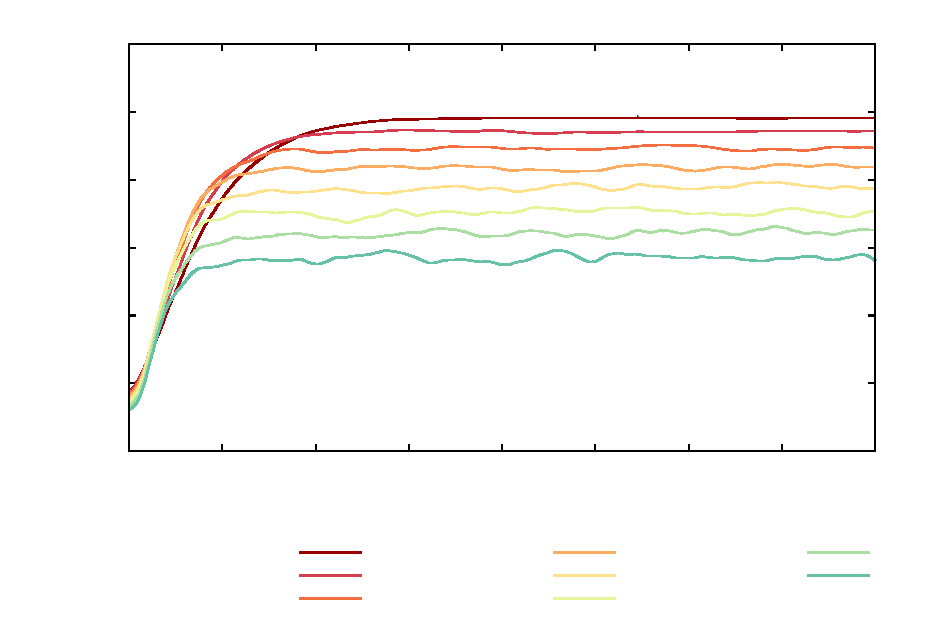
\includegraphics{figures/forcing/xhel_normed_128}}%
    \gplfronttext
  \end{picture}%
\endgroup
}
					\caption{\footnotesize{The average alignment over time is shown for different
                    forcing parameters $\sigma_{c,f}$.}}
					\label{test_normed_xhelicity_128}
				\end{figure}

            \end{minipage}
            \hfill
            \begin{minipage}[t]{20cm}

                In case of a strong alignment the dynamical effect also be seen in the
                Elsässer formulation of the incompressible MHD equations,

                \begin{equation}
                    \begin{aligned}
                    \label{elsasser_eq}
                    \va{z}^{\pm} = &\va{v} \pm \va{B},\\
                    \nabla \cdot \va{z}^{\pm} = &0\\
                    \frac{\partial}{\partial t} \va{z}^{\pm} + (\va{z}^{\mp}\cdot
                    \nabla)\va{z}^{\pm} = &-\nabla P + \frac{\nu + \lambda}{2}\Delta
                    \va{z}^{\pm} \\
                    &+ \frac{\nu - \lambda}{2}\Delta \va{z}^{\pm},
                    \end{aligned}
                \end{equation}

                where the non-linear term vanishes for $\va{z}^{\pm} \approx 0$.
                By reducing the non-linear interaction, the energy injected on
                large scales is transport less effienctly to smaller scales.

				\plot{figures/forcing/xhel_test_energy_flux_normed_t_05}
				{MHD stochastic forcing, dependency of energy dissipation evolution on cross helicity on .}
				{xhel_energy_dissipation_128}

            \end{minipage}
       }

		\block{Line element statistics}{

            \begin{minipage}[t]{20cm}

                \subheader{Strechting rates}

                The line element stretching rate was computed for each
                Lagrangian particle using Equation (\ref{zeta}) and 
                averaged over the ensemble. Further, the alignement 
                of the line elements with the principal strain rates was studied
                by finiding the eigenvectors of the strain rate tensor.
                
                \plot{figures/mhd_line_evo}
                    {Temporal evolution of the average line strechting rate and
                    orienation.}
                    {line_stretching}

                \begin{itemsposter}
                    \item After an initial transition phase the strechting rates
                        settle into a stationary state.

                    \vspace{0.5cm}

                    \item In this transition phase the line elements $\va{l}$ show
                        a strong alignment with the maximum postive strain direction
                        $\va{T}_1$.
                \end{itemsposter}

                \subheader{Orientation}

                The histograms for different angles between the line elements and the
                principal strain rates as well as the vorticity and magnetic field in the
                stationary state are shown below .

                \plot{figures/histograms/mhd_angle_histo_t20}
                    {MHD p.d.fs for the angles between the local magnetic field and the
                    line element orientation at steady state ($t/\tau_{\eta} = 20$).}
                    {mhd_strain_magnetic_angle_histo}

                \begin{itemsposter}
                    \item In MHD turbulence the line elements show the strongest
                        alignenment with the magnetic field, followed by the 
                        vorticity and the max. positive strain rate.
                \end{itemsposter}


            \end{minipage}
            \hfill
            \begin{minipage}[t]{20cm}

                 \subheader{Statistical distribution}
                    
                    The statistical distribution of the line element strechting
                    rate $\zeta$ was calculated in the stationary state. 

                    \plot{figures/histograms/mhd_zeta_histo_t20}
						{Probability density functions of $\zeta$ are shown for
                        different alignments $\langle \sigma \rangle$.}
						{histo}

                    \begin{itemsposter}
                        \item The p.d.f of $\zeta $ show
                              a Gaussian shaped distribution and are stationary.

                        \vspace{0.5cm}

                        \item The kurtosis of the p.d.f increases with an increasing
                              cross helicity fraction.
                    \end{itemsposter}


                 \subheader{Influence of the cross helicity}

                     After aligning $\va{v}$ and $\va{B}$ through cross helictiy
                     injection, its effect on material line stretching was
                     investigated by averaging the ensemble line stretching
                     rate and orientation over time for different alignments $\langle
                     \sigma_c \rangle $.

                    \plot{figures/line_xhel_scaling_128}
						{Time averaged stretching rates and angles are shown for
                        different alignment $\langle \sigma_c \rangle$.}
						{xhel_scaling}

                    \begin{itemsposter}
                        \item The stretching rate $\bar{\zeta}$ increases with
                            increasing alignment $\langle \sigma_c \rangle$.

                        \vspace{0.5cm}

                    \item At the same time the angle between $\va{l}$ and
                        $\va{T}_1$ or $\va{B}$ decreases with
                            increasing $\langle \sigma_c \rangle$.

                    \end{itemsposter}

                
            \end{minipage}
         
        }
	
	\end{columns}
	
\end{document}
